
\section{Calculations \& Graphs}

\vspace{-0.5cm}
\singlespacing

%------- Force --------%

\subsection{Force \& Acceleration} 

{\centering
\begin{equation}
	F = ma 
	\label{eq:NetForce}
\end{equation}
\begin{equation}
	a = \frac{F}{m} 
	\label{eq:CalculatedAcc}
\end{equation}
\begin{align*}
	\boldsymbol{F} &: \text{Force of object} \\
	\boldsymbol{m} &: \text{mass of object} \\
	\boldsymbol{a} &: \text{acceleration of object}
\end{align*}}

\subsubsection{Sample Calculation \\ {\normalfont \small\textit{Force of hanging mass at 10\,grams}}}

{\centering
\text{\textbf{Knowns:}}
\begin{align*}
	m &= \boldsymbol{.01\,\text{\textbf{kg}}} \\
	a &= \boldsymbol{9.8\,\text{\textbf{m/s}}^2}
\end{align*}

\text{\textbf{Calculating Force of Hanging Mass:}}
\begin{align*}
	F &= ma \\
	&= (.01)(9.8) \\
	F &= \boxed{0.098\,\text{N}}
\end{align*}}

\subsubsection{Sample Calculation \\ {\normalfont \small\textit{Acceleration of glider when hanging mass at 10 grams}}}

{\centering
\text{\textbf{Knowns:}}
\begin{align*}
	F &= \boldsymbol{0.098\,\text{\textbf{N}}} \\
	m &= \boldsymbol{0.3409\,\text{\textbf{kg}}}
\end{align*}

\text{\textbf{Calculating Expected Acceleration of Glider:}}
\begin{align*}
	a &= \frac{F}{m} \\
	&= \frac{0.098}{0.3409} \\
	a &= \boxed{0.2874\,\text{m/s}^2}
\end{align*}}


\newpage
%------- ACCELERATION BETWEEN TWO POINTS WITH INITIAL VELOCITY CLOSE TO ZERO--------%

\subsection{Acceleration Between Two Points with Initial Velocity Close to Zero} 

{\centering
\begin{equation}
	a = \frac{2\Delta{x}}{t^2} 
	\label{eq:MeasuredAcc}
\end{equation}
\begin{align*}
	\boldsymbol{\Delta{x}} &: \text{Distance between photogates} \\
\boldsymbol{t} &: \text{average time between photogates}
\end{align*}}

\subsubsection{Sample Calculation \\ {\normalfont \small\textit{Measured acceleration of glider with hanging mass at 10 grams}}}

{\centering
\textbf{Knowns:}
\begin{align*}
	\Delta{x} &= \boldsymbol{0.669\,\text{\textbf{m}}} \\
	t &= \boldsymbol{2.058\,\text{\textbf{s}}}
\end{align*}

\textbf{Calculating Measured Acceleration of Glider:}
\begin{align*}
	a &= \frac{2\Delta{x}}{t^2} \\
	&= \frac{(2)(0.669)}{(2.058)^2} \\
	a &= \boxed{0.3156\,\text{m/s}^2}
\end{align*}}

%------- ACCELERATION BETWEEN TWO POINTS --------%

%------- AVERAGE VALUE --------%
\subsection{Average Value Formula} 

\begin{align*}
	\overline{a} = \frac{\text{sum of values}}{\text{total \# of values}} 
\end{align*}

\subsubsection{Sample Calculation \\ {\normalfont \small\textit{average time between photogates of glider with hanging mass at 10 grams }}}


\begin{align*}
	\overline{a}&=\frac{\text{sum of values}}{\text{total \# of values}} \\ \\
							&= \frac{2.043+2.067+2.067}{3} \\ \\
	\overline{a}&= \boxed{2.059\,\text{s}}
\end{align*}
%------- AVERAGE VALUE --------%

%------- STANDARD DEVIATION --------%
\subsection{Standard Deviation Formula}

\begin{align*}
		\sigma &= \sqrt{\frac{\Sigma(x_i -\overline{a})^2}{N}} \\
		 &= \sqrt{\frac{SS}{N}} \\ \\
		\textbf{N} &:\, \text{Total number of values} \\
		\overline{\textbf{a}} &:\, \text{Average value} \\
		\textbf{x\textsubscript{i}} &:\, \text{Each value from the data set} \\
		\textbf{SS} &:\, \text{Sum of squares} 
\end{align*}

\subsubsection{Sample Calculation \\ {\normalfont \small\textit{std of photogate times with hanging mass at 10 grams }}}

\begin{align*}
	\sigma &= \sqrt{\frac{(2.043-\overline{a})^2 + ... + (2.067-\overline{a})^2}{3}} \\
		 &= \sqrt{\frac{0.000384}{3}} \\
		 &= \boxed{0.01131\, \text{s}}
\end{align*}
%------- STANDARD DEVIATION --------%

%------- RELATIVE ERROR --------%
\subsection{Relative Error Formula}

\begin{align*}
	RE &= \left| {\frac{V_A-V_E}{V_E}} \right|\: \text{x}\: 100\% \\ \\
	\boldsymbol{V_A} &:\, \text{Actual value observed} \\
	\boldsymbol{V_E} &:\, \text{Expected value} 
\end{align*}

\subsubsection{Sample Calculation \\ {\normalfont \small\textit{acceleration of glider on air track with hanging mass at 10 grams - measured vs calculations}}}

\begin{align*}
	RE &= \left| {\frac{V_A-V_E}{V_E}} \right|\: \text{x}\: 100\% \\
	 &= \left| {\frac{0.3156-0.2874}{0.2874}} \right|\: \text{x}\: 100\% \\
			RE &= \boxed{9.80\%} 
\end{align*}
%------- RELATIVE ERROR --------%

%----TABLES-----%

\begin{landscape}

\subsection{Tables}

\begin{table}[H]
\captionsetup{font=Large}
\caption{Known values}
\centering
\begin{threeparttable}
\resizebox{\textwidth}{!}{%
\begin{tabular}{ccccc}
	\textbf{g$\boldsymbol{(\text{\textbf{m/s}}^2})$} & $\boldsymbol{x_1\text{\textbf{(m)}}}\tnote{!}$ & $\boldsymbol{x_2\text{\textbf{{(m)}}}}\tnote{!}$ & $\boldsymbol{\Delta{x}\text{\textbf{(m)}}}$ & \textbf{M(m)\tnote{!!}} \\ \hline
9.80 & 1.169 & 0.5 & 0.669 & 0.3409
\end{tabular}%
}
\begin{tablenotes}\normalsize
	\item[!] Positions of photogates 1 and 2
	\item[!!] Mass of entire system
\end{tablenotes}
\end{threeparttable}
\label{tab:knownsTab}
\end{table}

\vspace{-0.5cm}

\begin{table}[H]
\captionsetup{font=Large}
\caption{Accelerating System of Mass M}
\centering
\begin{threeparttable}
\resizebox{\columnwidth}{!}{%
\begin{tabular}{ccccccccc}
\textbf{Measurement \#}         & 1       & 2      & 3       & 4        & 5        & 6       & 7      & 8       \\ \hline
\textbf{m (g)\tnote{!}}                   & 0.01    & 0.015  & 0.02    & 0.025    & 0.03     & 0.035   & 0.04   & 0.045   \\
\textbf{$\boldsymbol{F_{\textbf{net}}}$ (N)}          & 0.098   & 0.147  & 0.196   & 0.245    & 0.294    & 0.343   & 0.392  & 0.441   \\
\textbf{a(expected) $\boldsymbol{(\textbf{m}/\textbf{s}^2)}$} & 0.2874  & 0.4312 & 0.5749  & 0.7186   & 0.8623   & 1.0060  & 1.1498 & 1.2935  \\
\textbf{$\boldsymbol{T_{1}}$ (s)}            & 2.043   & 1.698  & 1.515   & 1.298    & 1.223    & 1.083   & 0.9914 & 0.9405  \\
\textbf{$\boldsymbol{T_{2}}$ (s)}            & 2.067   & 1.732  & 1.435   & 1.316    & 1.223    & 1.075   & 1.045  & 0.9811  \\
\textbf{$\boldsymbol{T _{3}}$ (s)}           & 2.067   & 1.739  & 1.491   & 1.298    & 1.207    & 1.143   & 1.037  & 1.008   \\
\textbf{$\boldsymbol{T _{\textbf{avg}}}$ (s)}         & 2.059   & 1.723  & 1.48    & 1.304    & 1.217    & 1.1     & 1.024  & 0.9765  \\
\textbf{$\boldsymbol{T _{\textbf{std}}}$ (s)}          & 0.01131 & 0.0179 & 0.03351 & 0.008485 & 0.007542 & 0.03034 & 0.0236 & 0.02774 \\
\textbf{a(measured) $\boldsymbol{(\textbf{m}/\textbf{s}^2)}$}  & 0.3156  & 0.4506 & 0.6108  & 0.7868   & 0.9033   & 1.105  & 1.276 & 1.403  \\ \hline
\textbf{Percent Error (\%)}   & 9.80    & 4.51   & 6.25    & 9.49     & 4.75     & 9.84    & 10.98  & 8.47    
\end{tabular}%
}
\begin{tablenotes}\normalsize
	\item[!] Hanging mass only 
\end{tablenotes}
\end{threeparttable}
\label{tab:dataTab}
\end{table}
\end{landscape}
 
%----TABLES-----%

%----GRAPHS-----%

\begin{landscape}
\subsection{Graphs}
\begin{figure}[H]
	\begin{center}
		\captionsetup{font=Large}
		\caption{Force vs. Acceleration}\label{fig:GFvA}
		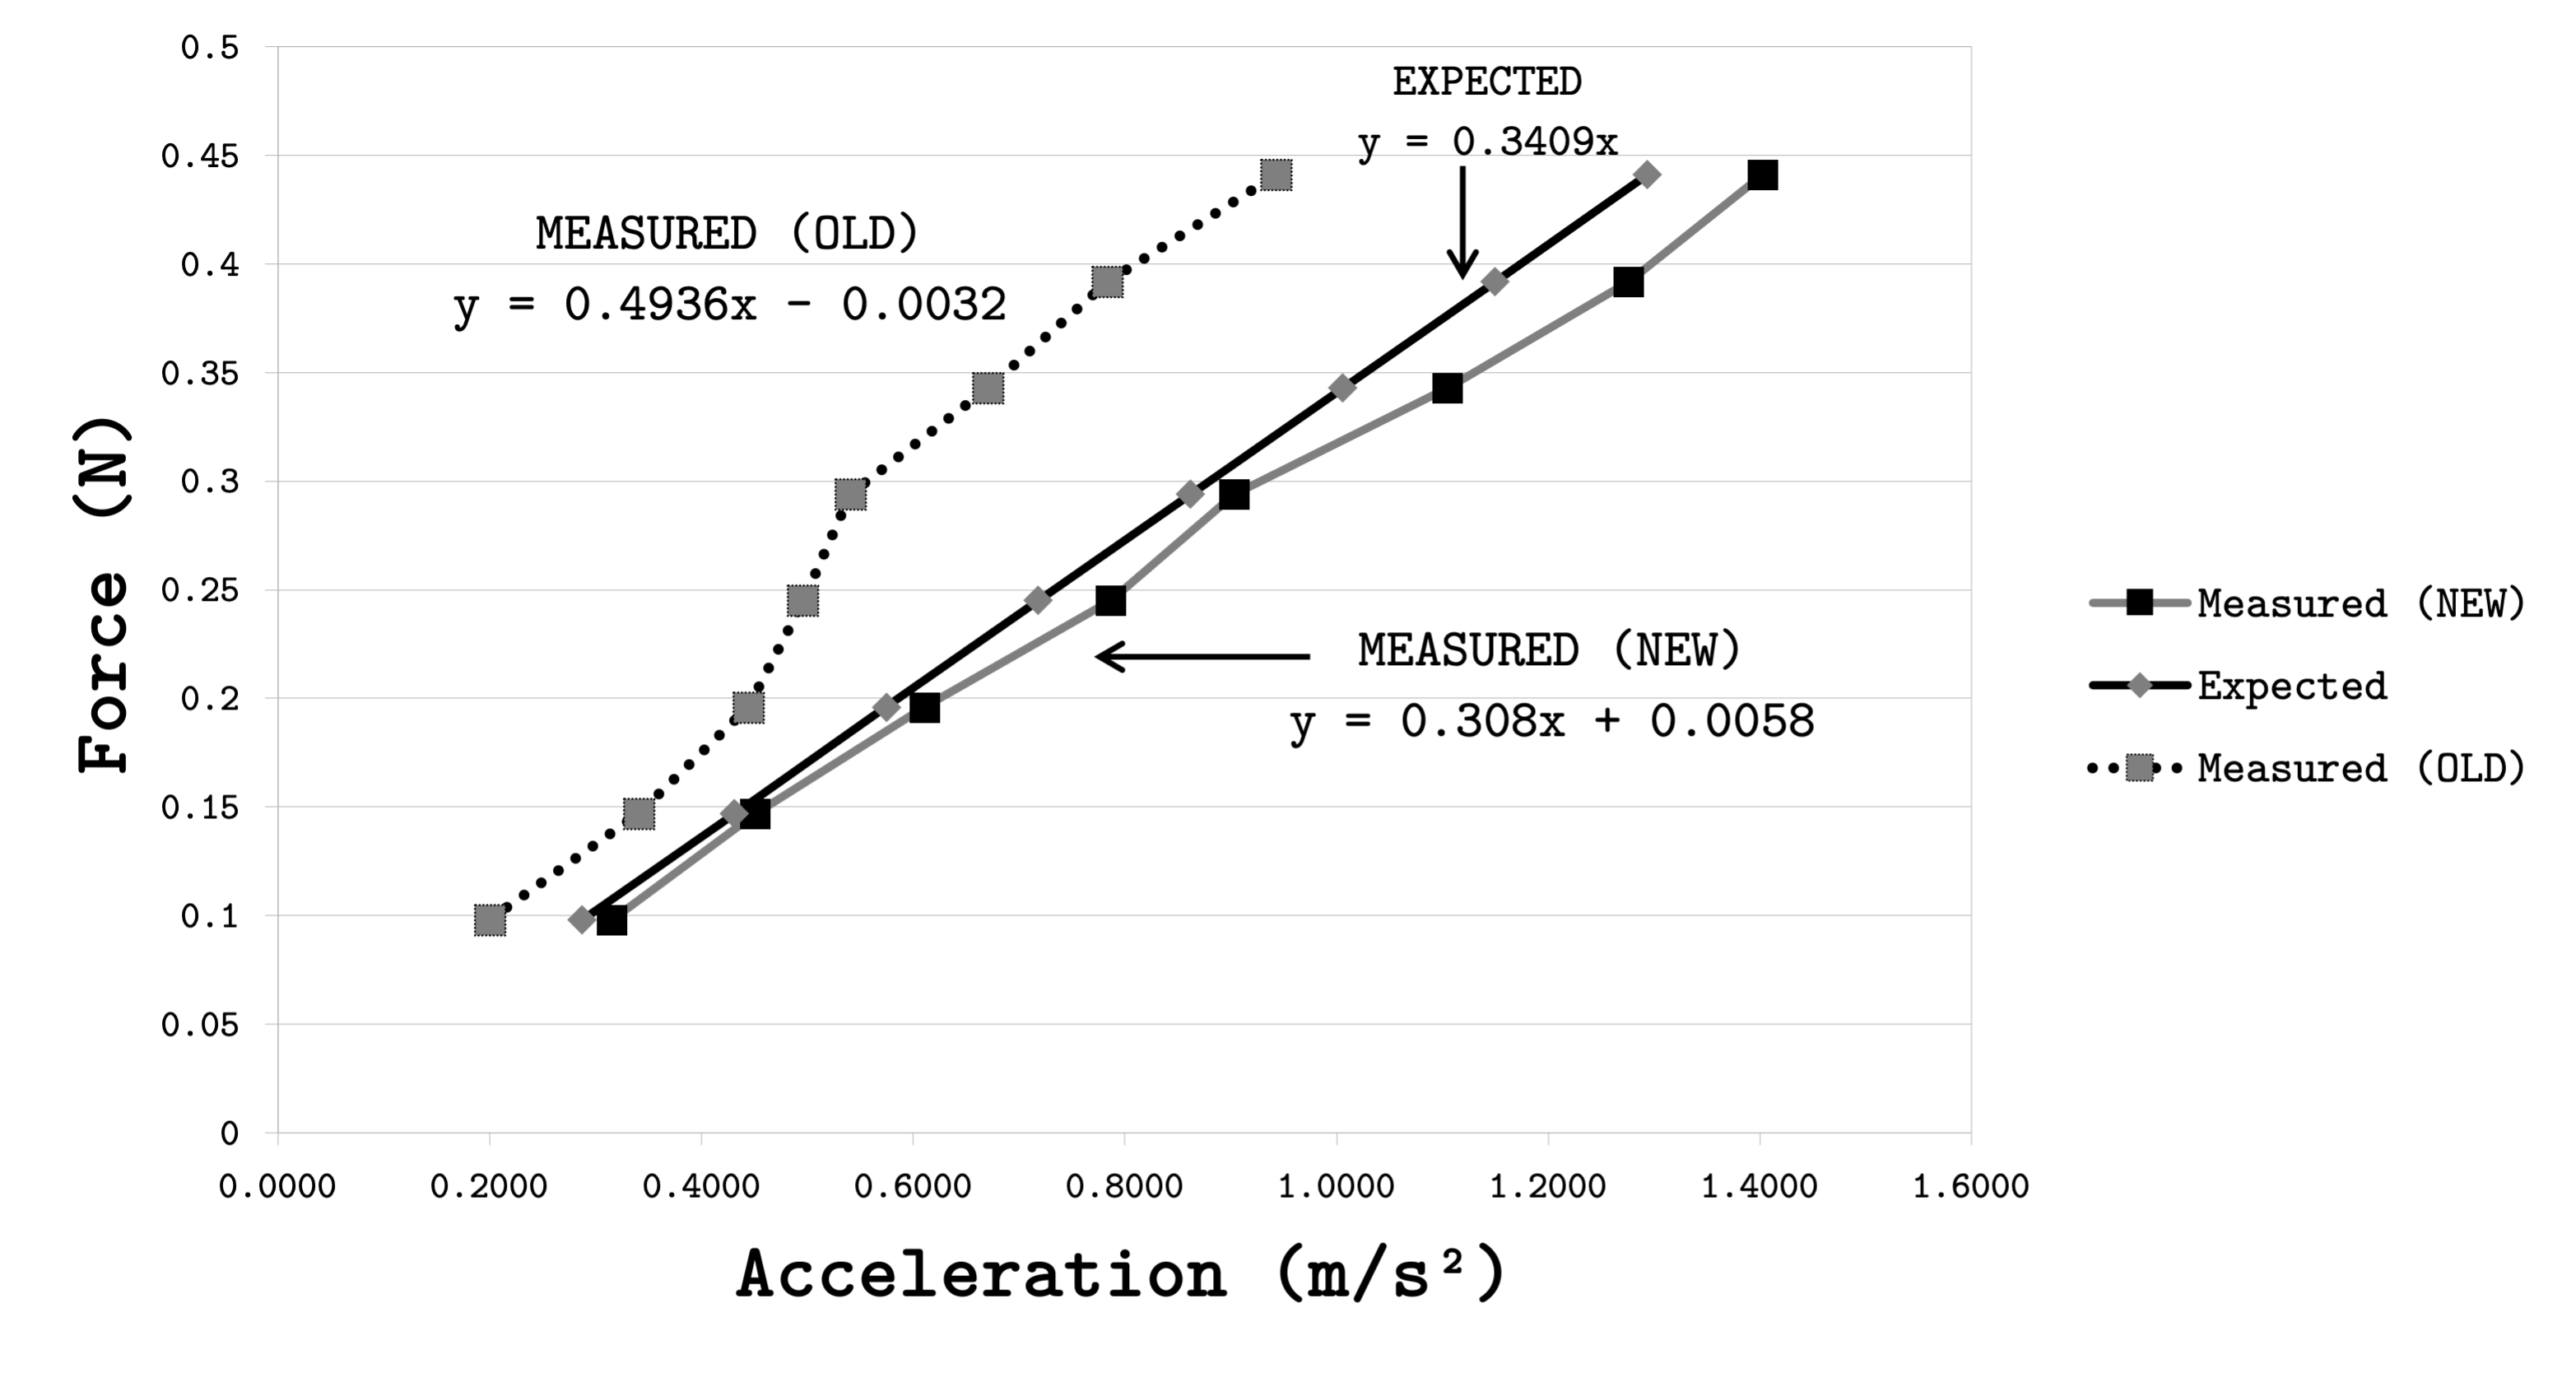
\includegraphics[width=0.90\columnwidth]{images/GraphFvA}
	\end{center}
\end{figure}
\end{landscape}

%----GRAPHS-----%

\newpage

